\section{Communicating Pick-and-Place}
\label{problem}

This section provides a formalization of pick-and-place tasks and identifies information required to specify them.
 
\noindent\textbf{Manipulator}: Robots that can physically interact with their surroundings are called \textit{manipulators}, of which robotic arms are the prime example. 

\noindent\textbf{Workspace}: The manipulator operates in a 3D workspace $\mathcal{W} \subseteq \mathbb{R}^3$. The workspace also contains a stable surface of interest defined by a plane $S\subset\mathcal{W}$ along with various objects. To represent 3D coordinates of workspace positions, we use $x\in\mathcal{W}$. 

\noindent\textbf{End-effector}: The \textit{tool-tips} or \textit{end-effectors} are geometries, often attached at the end of a robotic arm, that can interact with objects in the environment. These form a manipulator's chief mode of picking and placing objects of interest and range from articulated fingers to suction cups. A subset of the workspace that the robot can \textit{reach} with its end-effector is called the reachable workspace. The end-effector in this work is used as a pointing indicator.

\noindent\textbf{Pick-and-place}: Given a target object in the workspace, a \textit{pick-and-place} task requires the object to be picked up from its initial position and orientation, and placed at a final position and orientation. When a manipulator executes this task in its reachable workspace, it uses its end-effector. 
The rest of this work ignores the effect of the object's orientation by considering objects with sufficient symmetry. Given this simplification, the pick-and-place task can be viewed as a transition from an initial position $\xinit\in\mathcal{W}$ to a final placement position $\xfinal\in\mathcal{W}$.  Thus, a pick-and-place task can be specified with a tuple
$$ \textit{PAP} = \langle o, \xinit, \xfinal \rangle. $$


\begin{figure}[t]
\centering
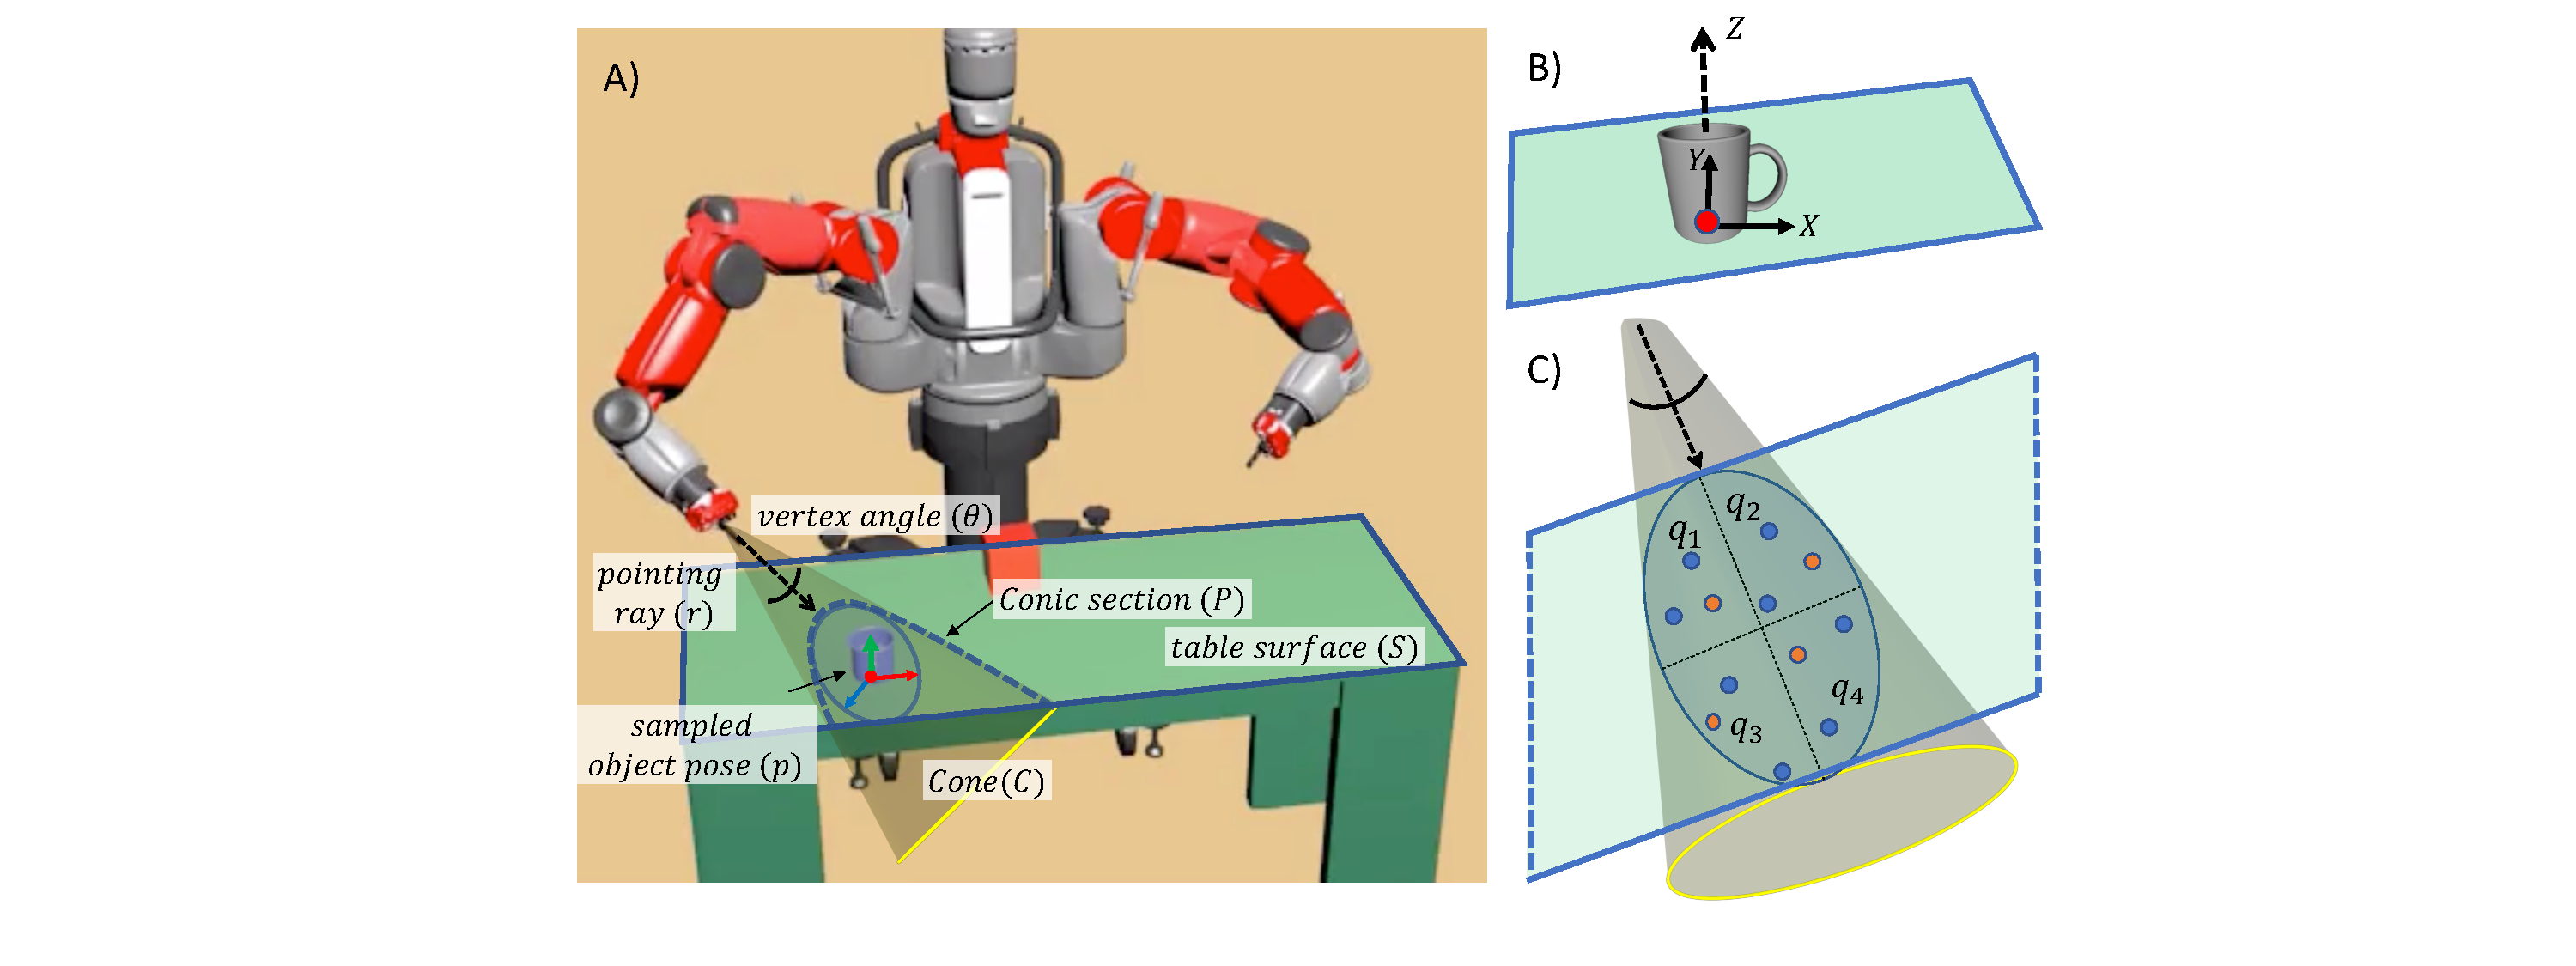
\includegraphics[width=0.5\textwidth]{pointing_diagram}
\caption{(A) Workspace setup showing the pointing cone and the corresponding conic section on the table. (B) The degrees-of-freedom considered for placement of the object on the table. (C) Sampling policy to sample object poses within the conic section.}
    \label{fig:pointing}
\end{figure}

\noindent\textbf{Pointing Action}: Within its reachable workspace the end-effector of the manipulator can attain different orientations to fully specify a reachable \textit{pose} $p$, which describes its position and orientation.  The robots we study have a directional tooltip that viewers naturally see as projecting a ray $r$ along its axis outward into the scene.  In understanding pointing as communication, the key question is the relationship between the ray $r$ and the spatial values $\xinit$ and $\xfinal$ that define the pick-and-place task.

% own on what it entails through our study.

To make this concrete, we distinguish between the \emph{target} of pointing and the \emph{intent} of pointing. Given the ray $r$ coming out of the end-effector geometry, we define the target of the pointing as the intersection of this ray on the stable surface, $$x^*= r\cap S.$$ Meanwhile, the intent of pointing specifies one component of a pick-and-place task.  There are two cases:
\begin{itemize}
    \item [-] \textit{Referential Pointing:} The pointing action is intended to identify a target object $o$ to be picked up. This object is the \textit{referent} of such an action. We can find $\xinit$, based on the present position of $o$.
    \item [-] \textit{Locating Pointing:} The pointing action is intended to identify the location in the workspace where the object needs to be placed, i.e, $\xfinal$.
\end{itemize}


We study effective ways to express intent for a pick-and-place task. In other words, what is the relationship between a pointing ray $r$ and the location $\xinit$ or $\xfinal$ that it is intended to identify?  To assess these relationships, we ask human observers to view animations expressing pick-and-place tasks and classify their interpretations.  To understand the factors involved, we investigate a range of experimental conditions.
